\section{Théorème de Thalès}
    \subsection{Énoncé}
        \begin{theoreme}[\admis]
            Si dans une configuration géométrique :
            \begin{itemize}
                \item Deux droites $(d)$ et $(d')$ sont sécantes en un point $A$.
                \item $B$ et $M$ sont deux points de la droites $(d)$, distincts de A.
                \item $C$ et $N$ sont 2 points de la droite $(d')$, distincts de $A$.
                \item les droites $(BC)$ et $(MN)$ sont parallèles.       
            \end{itemize}
            \medskip
            alors les rapports $\dfrac{AM}{AB}$ , $\dfrac{AN}{AC}$ et $\dfrac{MN}{BC}$ sont égaux.
        \end{theoreme}

        \begin{remarque}
            En fait ce théorème traduit la proportionnalité entre les longueurs des côtés des triangles $ABC$ et $AMN$.

            Les rapports $\dfrac{AB}{AM}$ , $\dfrac{AC}{AN}$ et $\dfrac{BC}{MN}$ sont donc aussi égaux.
        \end{remarque}
    
    \subsection{Configurations de Thalès}
        \emoji{light-bulb} \color{red}{\dashuline{\color{black}{Les droites en pointillés rouges sont parallèles.}}}
        \color{black}

        \hspace*{-1cm}
        % \vspace*{-4cm}
        \begin{tikzpicture}[scale = 0.5]        
            % \draw[help lines, color=black!30, dashed] (0,0) grid (12,14);        
            \coordinate[label=left:$A$] (A) at (7,13);
            \coordinate[label=left:$(d')$] (d') at (6.5,15);
            \coordinate[label=right:$(d)$] (d) at (8,15);
            \coordinate[label=above right:$C$] (C) at (10,1);
            \coordinate[label=above left:$B$] (B) at (1,1);
            \coordinate[label=above left:$M$] (M) at (5,9);
            \coordinate (M1) at (2,9);
            \coordinate[label=above right:$N$] (N) at (8,9);
            \coordinate (N1) at (11,9);

            \tkzDrawLine(A,B);
            \tkzDrawLine(A,C);
            \tkzDrawLine(B,C);        
            \tkzDrawLine(M1,N1);
            \tkzDrawLine[dashed, color=red, ultra thick](M1,N1);
            \tkzDrawLine[dashed, color=red, ultra thick](B,C);
        \end{tikzpicture}
        \begin{tikzpicture}[scale = 0.5]
            % \draw[help lines, color=black!30, dashed] (0,0) grid (12,14);        
            \coordinate[label=left:$A$] (A) at (7,13);
            \coordinate[label=left:$(d')$] (d') at (6.7,14);
            \coordinate[label=right:$(d)$] (d) at (7.5,14);
            \coordinate[label=above right:$N$] (N) at (9,5);
            \coordinate[label=above left:$M$] (M) at (3,5);
            \coordinate[label=above left:$B$] (B) at (5,9);
            \coordinate (M1) at (4,5);
            \coordinate[label=above right:$C$] (C) at (8,9);
            \coordinate (N1) at (10,5);

            \tkzDrawLine(A,M);
            \tkzDrawLine(A,N);
            \tkzDrawLine(M,N);
            \tkzDrawLine(B,C);
            \tkzDrawLine(M1,N1);     
            \tkzDrawLine[dashed, color=red, ultra thick](M1,N1);
            \tkzDrawLine[dashed, color=red, ultra thick](B,C);
        \end{tikzpicture}
        \begin{tikzpicture}[scale = 0.5]
            % \draw[help lines, color=black!30, dashed] (0,0) grid (12,18);        
            \coordinate[label=left:$A$] (A) at (7,13);
            \coordinate[label=right:$(d)$] (d) at (9.5,18);
            \coordinate[label=left:$(d')$] (d') at (5.7,18);
            \coordinate[label=above right:$C$] (C) at (10,1);
            \coordinate[label=above left:$B$] (B) at (1,1);
            \coordinate[label=below right:$M$] (M) at (9,17);
            \coordinate (M1) at (3,17);
            \coordinate[label=below left:$N$] (N) at (6,17);
            \coordinate (N1) at (12,17);

            \tkzDrawLine(N,C);
            \tkzDrawLine(M,B);
            \tkzDrawLine(B,C);
            \tkzDrawLine(M1,N1);     
            \tkzDrawLine[dashed, color=red, ultra thick](M1,N1);
            \tkzDrawLine[dashed, color=red, ultra thick](B,C);
        \end{tikzpicture}

    \subsection{Exemple de rédaction}

        \begin{methode*1}[Calculer une longueur]
            \begin{multicols}2
                \begin{itemize}
                    \item Déterminer les droites sécantes.
                    \item Déterminer les droites parallèles,
                    
                    éventuellement le justifier.
                    \item Identifier les deux triangles.                    
                    \item Écrire l'égalité des trois rapports.
                    \item Déterminer les longueurs inconnues.
                \end{itemize}
            \end{multicols}

            \exercice

            \begin{minipage}{8cm}
                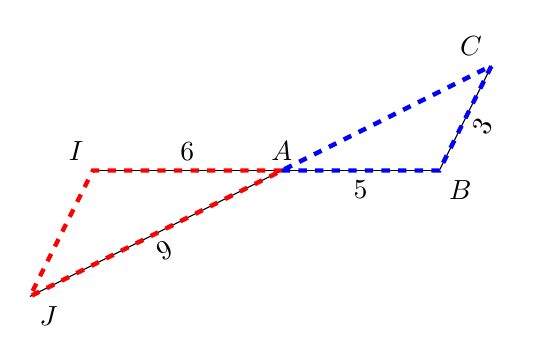
\begin{tikzpicture}[scale = 0.4]
                    % \draw[help lines, color=black!30, dashed] (0,0) grid (18,12);                    
                    \coordinate (J1) at (1,1);
                    \coordinate (I1) at (6,11);
                    \tkzDrawLine(J1,I1);

                    \coordinate (B1) at (12,1);
                    \coordinate (C1) at (17,11);
                    \tkzDrawLine(B1,C1);

                    \coordinate[label=above left:$I$] (I) at (4,7);
                    \coordinate[label=below right:$B$] (B) at (15,7);            
                    \tkzDrawLine(I,B);
                    

                    \coordinate[label=below right:$J$] (J) at (2,3);
                    \coordinate[label=above left:$C$] (C) at (16.66,10.33);
                    \tkzDrawLine(J,C);

                    \coordinate[label=above:$A$] (A) at (10,7);
                    \draw (I) -- node[sloped,above] {\Lg{6}} (A) -- node[sloped,below] {\Lg{5}} (B);
                    \draw (J) -- node[sloped,below] {\Lg{9}} (A);
                    \draw (B) -- node[sloped,below] {\Lg{3}} (C);

                    \draw[dashed, color=red, ultra thick] (A) -- (I) -- (J) -- (A);
                    \draw[dashed, color=blue, ultra thick] (A) -- (B) -- (C) -- (A);
                \end{tikzpicture}
            \end{minipage}
            \begin{minipage}{8cm}
                \begin{itemize}
                    \item Les droites $(CJ)$ et $(BI)$ se coupent en $A$.
                    \item Les droites $(BC)$ et $(IJ)$ sont parallèles.
                \end{itemize}
                Calculer les longueurs $AC$ et $IJ$.
            \end{minipage}
            
            \correction
            Dans la configuration ci-dessus : 
            \begin{itemize}
                \item les droites $(CJ)$ et $(BI)$ sont sécantes en $A$.
                \item les droites $(IJ)$ et $(BC)$ sont parallèles.
                \item les deux triangles de la configurations sont \textcolor{red}{$AIJ$} et \textcolor{blue}{$ABC$}.
            \end{itemize}
            D'après le théorème de Thalès, on peut donc écrire l'égalité des trois rapports :
            $$\frac{\textcolor{red}{AI}}{\textcolor{blue}{AB}}=\frac{\textcolor{red}{AJ}}{\textcolor{blue}{AC}}=\frac{\textcolor{red}{IJ}}{\textcolor{blue}{BC}}\qquad\mbox{c'est à dire}\qquad\frac{\textcolor{red}{6}}{\textcolor{blue}{5}}=\frac{\textcolor{red}{9}}{\textcolor{blue}{AC}}=\frac{\textcolor{red}{IJ}}{\textcolor{blue}{3}}$$

            \begin{minipage}{8cm}
                $$\mbox{\bf Pour le calcul de AC}$$
                $$\mbox{on utilise} \quad \dfrac{6}{5}=\dfrac{9}{AC}$$
                \begin{center}
                    {\bf Les produits en croix sont égaux}
                \end{center}
                $$\Eqalign{6\times AC&=9\times5}$$
                \begin{center}
                    {\bf On divise les deux membres par 6}
                \end{center}
                $$\Eqalign{AC&=\frac{9\times5}{6}=\Lg{7.5}\cr}$$
            \end{minipage}
            \vrule
            \begin{minipage}{8cm}
                % \begin{leftbar}
                $$\mbox{\bf Pour le calcul de IJ}$$
                $$\mbox{on utilise} \quad \dfrac{6}{5}=\dfrac{IJ}{3}$$
                \begin{center}
                    {\bf Les produits en croix sont égaux}
                \end{center}
                $$\Eqalign{5\times IJ&=6\times3}$$
                \begin{center}
                    {\bf On divise les deux membres par 5}
                \end{center}
                $$\Eqalign{IJ&=\frac{6\times3}{5}=\Lg{3.6}\cr}$$
                % \end{leftbar}
            \end{minipage}
        \end{methode*1}


% \subsection{Sous-section 1.1}
% \begin{definition}[Titre optionnel]
%     Dans le cours, on utilise assez souvent des cadres du type
%     définition (comme ici par exemple).    
% \end{definition}
% \begin{remarque}
%     Ceci est une remarque utilisant une commande du paquet profcollege.
    
%     \begin{center}
%       Truc centré
%     \end{center}


% \end{remarque}
% \begin{propriete}[Titre optionnel]
%   Dans le cours, on utilise assez souvent des cadres du type
%   définition, comme ici par exemple pour une propriete.
% \end{propriete}
% \begin{remarques}
%   \begin{itemize}
%     \item remarque.
%     \item remarque.
%   \end{itemize}
% \end{remarques}

% \subsection{Sous-section 1.2}
% \begin{theoreme}[Titre optionnel]
%   Dans le cours, on utilise assez souvent des cadres du type
%   définition, comme ici par exemple pour un théorème.
% \end{theoreme}
% \begin{notation}
%   notation
% \end{notation}
% \begin{notations}
%   \begin{itemize}
%     \item notation.
%     \item notation.
%   \end{itemize}
% \end{notations}
% \begin{preuve}
%   Ceci est une preuve\par Deuxième ligne de la preuve
% \end{preuve}
% \begin{exemple}
%   Texte de l’exemple
%   \correction
  
% \end{exemple}

% \begin{exemple*1}
%   \phantom{rrr}
%   Texte

%   \correction
%   \phantom{rrr}
%   Texte  
  
% \end{exemple*1}

% \begin{exemple}[0.6]
%   Texte de l’exemple très long sur une ligne, très très très long.
%   On peut modifier la répartition horizontale  à l'aide d'un argument optionnel valant par défaut 0,4, valant ici 0,6.
%   \correction
%   Texte de la correction en vis à vis
% \end{exemple}
% \section{Section 2}
% \subsection{Sous-section 2.1}
% Quatre affichages prévus pour les méthodes.

% \begin{methode}[Titre de la méthode]
%     \Papiers[Largeur=10,Hauteur=5,Couleur=Olive]
    
%     Texte introductif
%     \exercice
%     Texte de l’exercice
%     \correction
%     Texte de la correction sur un minimum de trois lignes pour faire la
%     différence entre vis-à-vis et double colonne. C’est l’endroit de la
%     coupure qui va différer.
% \end{methode}

% \begin{methode*1}[Titre de la méthode*1]
%     Texte introductif
%     \exercice
%     Texte de l’exercice
%     \correction
%     Texte de la correction sur un minimum de trois lignes pour faire la
%     différence entre vis-à-vis et double colonne. C’est l’endroit de la
%     coupure qui va différer.
% \end{methode*1}

% \subsection{Sous-section 2.2}
% \begin{methode*2}[Titre de la méthode*2]
%     Texte introductif
%     \exercice
%     Texte de l’exercice
%     \correction
%     Texte de la correction sur un minimum de trois lignes pour faire la
%     différence entre vis-à-vis et double colonne. C’est l’endroit de la
%     coupure qui va différer.
% \end{methode*2}

% \begin{methode*2*2}[Dernière méthode  \MethodeRefExercice{exoN1-exemple1} \MethodeRefExercice{exoN1-exemple2}]
%     \exercice
%     \label{methodeN1-exemple}
%     Texte du premier exercice
%     \correction
%     Correction du premier exercice
%     \exercice
%     Texte du deuxième exercice
%     \correction
%     Texte de la correction du deuxième exercice sur un minimum de trois
%     lignes pour faire la différence entre vis-à-vis et double
%     colonne. C’est l’endroit de la coupure qui va différer.
% \end{methode*2*2}